\documentclass{article}

\usepackage{tikz}

\renewcommand\figurename{Figura}

\definecolor{rosu}{rgb}{0.9, 0.17, 0.31}
\definecolor{albastru}{rgb}{0.2, 0.2, 0.6}

\begin{document}

\subsection{Breviar teoretic}

{\color{albastru}
Fie $G$ un graf orientat. $G$ este un \textit{arbore cu rădăcina $r$}, dacă există $G$ un vârf $r$ din care oricare alt vârf poate fi ajuns printr-un drum unic.

Definiţia este valabilă şi pentru cazul unui graf neorientat, alegerea unei rădăcini fiind însă în acest caz arbitrară: orice arbore este arbore cu rădăcină, iar rădăcina poate fi fixată în oricare vârf al său. Aceasta, deoarece dintr-un vârf oarecare se poate ajunge în oricare alt vârf printr-un drum unic.
}

\begin{figure}[h]
\begin{minipage}[t]{.3\textwidth}
	\begin{tabular}{c c}
		nivelul & adâncimea \\[.1cm]
		2 & 0 \\[1.4cm]
		1 & 1 \\[1.4cm]
		0 & 2
	\end{tabular}
\end{minipage}%
\begin{minipage}[c]{.3\textwidth}
	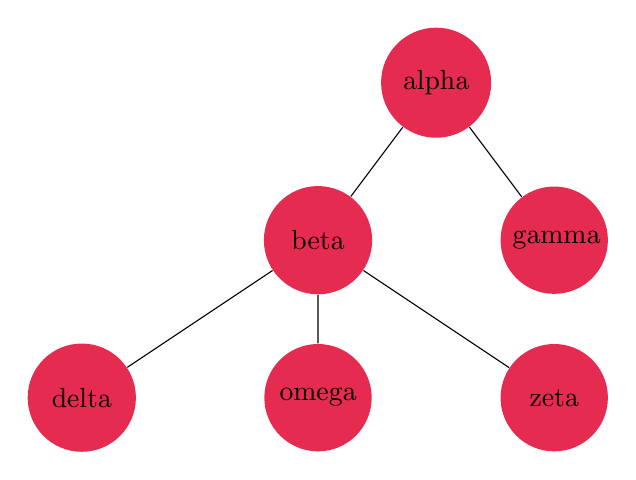
\begin{tikzpicture}[
		level/.style={sibling distance=3cm, level distance=2cm},
		every node/.style = {align=center, text width=3em, shape=circle, fill=rosu }]
		\node{alpha}
			child{ node {beta}
				child{ node {delta} }
				child{ node {omega} }
				child{ node {zeta} }
			}
			child{ node {gamma} };
	\end{tikzpicture}
\end{minipage}
\caption{Un arbore cu rădăcină} \label{fig:arbore}
\end{figure}

{\color{albastru} Când nu va fi pericol de confuzie, vom folosi termenul "arbore", în loc de termenul corect "arbore cu rădăcină". Ce mai intuitiv este să reprezentăm un arbore cu rădăcină, ca pe un arbore propriu-zis. În figura \ref{fig:arbore}, vom spune că \textit{beta} este \textit{tatăl} lui \textit{delta} şi fiul lui \textit{alpha}, că \textit{beta} şi \textit{gamma} sunt \textit{fraţi}, că \textit{delta} este un \textit{descendent} al lui \textit{alpha}, iar \textit{alpha} este un \textit{ascendent} al lui \textit{delta}.}

\end{document}
